\chapterimage{chapter_head_1.pdf} 
\chapter{Programación de un juego sin gráficos}

En este capítulo, se darán las instrucciones para la realización paso a paso un videojuego sin usar el sistema gráfico de la NDS.

La lista de ejercicios y el tiempo estimado (en minutos) para su realización se muestran en la Tabla \ref{c4_tab:ejercios}.

\begin{table}[t]
\centering
\caption{Ejercicios del capítulo y tiempo estimado para su realización.}
\begin{tabular}{|c|c|}
\hline 
Ejercicio & Tiempo  \\ 
\hline 
 4.1 &   \\ 
 4.2 &   \\ 
 4.3 &    \\ 
 4.4 & \\ 
 4.5 & \\ 
 4.6 & \\ 
 4.7 & \\ 
 4.8 & \\ 
 4.9 & \\ 
 4.10 & \\
\hline 
\end{tabular} 
\label{c4_tab:ejercios}
\end{table}
% ---------------------------------------------------------
% ---------------------------------------------------------
\section{Descripción del juego}
El juego que se va a realizar será una versión del típico juego de carreras de caballos que se solían encontrar en las ferias itinerantes. La Figura \ref{fig_c4_caballos}\footnote{La imagen se ha obtenido en la siguiente web: \url{http://www.parquedebolas.com/images/productos/gran/523000002.jpg}} muestra un ejemplo de este tipo de juego. En este juego, el usuario debe introducir bolas en unos agujeros, y según el agujero donde ha caído la bola, el caballo irá más o menos deprisa. Gana el caballo que antes llegue a la meta.

Hola

\begin{figure}[t]
	\centering
	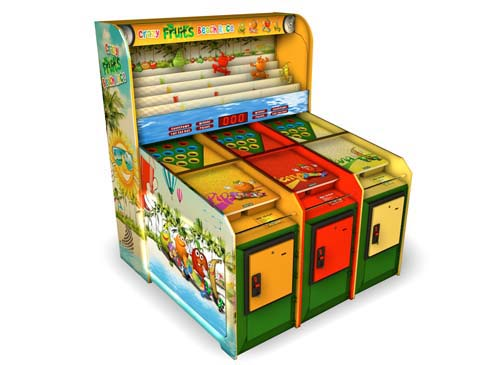
\includegraphics[height=7cm]{Figuras/C4/c4_caballos.jpg}
	\caption{Juego de las carreras de caballos.}
	\label{fig_c4_caballos}
\end{figure}

En la versión que se va a desarrollar se usarán los conceptos aprendidos en el cápitulo 3. En la pantalla superior se mostrará la carrera. La pantalla se dividirá en 4 carriles horizontales, uno por caballo. El caballo del jugador será siempre el situado en el carril superior. Para representar cada caballo se usará una letra. Al inicio los 4 caballos se situarán en la primera columna de la pantalla (columna 0). El objetivo es desplazar el caballo hacia la derecha lo más rápido que sea posible. Ganará el primer caballo que alcance la meta situada en la última columna de la pantalla (columna 31).

La pantalla inferior será el espacio donde el jugador interactuará para conseguir que se caballo gane. La pantalla inferior se dividirá en una rejilla de 16x16 celda. Por lo tanto, cada celda tendrá una dimensión de 12x16 píxeles de la pantalla táctil. De forma aleatoria, una celda se iluminará. Si el jugador pulsa sobre dicha celda en el momento correcto, su caballo aumentará la velocidad, en caso contrario la velocidad del caballo disminuirá. Para simular la iluminación de una celda, se usará el caracter X.

En el aula virtual se encuentra el ejecutable del programa una vez acabado.

El siguiente listado (\textit{caballos\_inicial.c}) muestra el esqueleto del programa que puedes usar para empezar:
\begin{lstlisting}
#include [...] 
int main(void)
{
	inicializar libNDS; 
	while(1){
		// Bucle principal 
	}
	return 0;
}
\end{lstlisting}

Para crear el programa completo debes resolver los siguientes ejercicios en el orden establecido.

\begin{exercise}
	Crea un nuevo proyecto usando el programa 
\end{exercise}

